\documentclass[10pt]{article}
\usepackage[utf8]{inputenc}
\usepackage{cite}
\title{Teoria dos Grafos}
\author{Pedro Meira-Betmann}
\date{November 2019}

\usepackage{natbib}
\usepackage{graphicx}
\usepackage{url}

\begin{document}

\maketitle

\section{Introdução}
A cadeira de teoria dos Grafos aborda, com ajuda de programação, os grafos que podem ser representados visualmente por vértices e arestas, que ligam tais vértices, e em geral procuram soluções para problemas reais como o problema de fluxo máximo que tenta determinar o limite superior de cada caminho e como utilizá-los usando métodos como programação linear, ou ate força bruta. Além disso, fatores facilitadores como o Google usam da teoria dos grafos combinado com outros fatores para fazer o ranqueamento das páginas em uma pesquisa, ao todo essa área abrange grande parte da computação e pode participar de qualquer projeto que utilize objetos que interagem entre si.

\begin{figure}[h!]
\centering
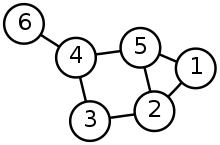
\includegraphics[scale=1]{graph.jpg}
\caption{grafo de 6 vértices e 7 arestas \cite{wiki:xxx}}
\label{fig:graph}
\end{figure}
\section{Relevância}
Na cadeira, os assuntos abordados em maior parte são otimização, tanto de códigos quanto problemas de otimização, aplicação de grafos em problemas e como podem ser usados, o último tema abordado na cadeira varia dependendo do professor e do ano, na cadeira atual o foco da última parte é a questão de p versus np que novamente se volta para otimização de tempo e memória.
\section{Relação com outras cadeiras}
\subsection{IF672 - Algoritmos e Estruturas de Dados}
O requerimento da cadeira de teoria dos grafos é algoritmos e estrutura de dados, onde se vê problemas np completos, otimização de códigos, estrutura de dados e algoritmos geométricos, os quais são importantes para manipular grafos de maneira eficiente \cite{curriculo}.
\subsection{IF670 - Matemática Discreta para Computação}
Essa cadeira disponibiliza a base para mexer com relações entre objetos e problemas de otimização.
\subsection{MA531 - Álgebra Vetorial Linear para Computação}
Essa cadeira apresenta os conceitos básicos necessários para programação linear, fator de extrema importância na cadeira de teoria dos grafos.
\begin{figure}[h!]
\centering
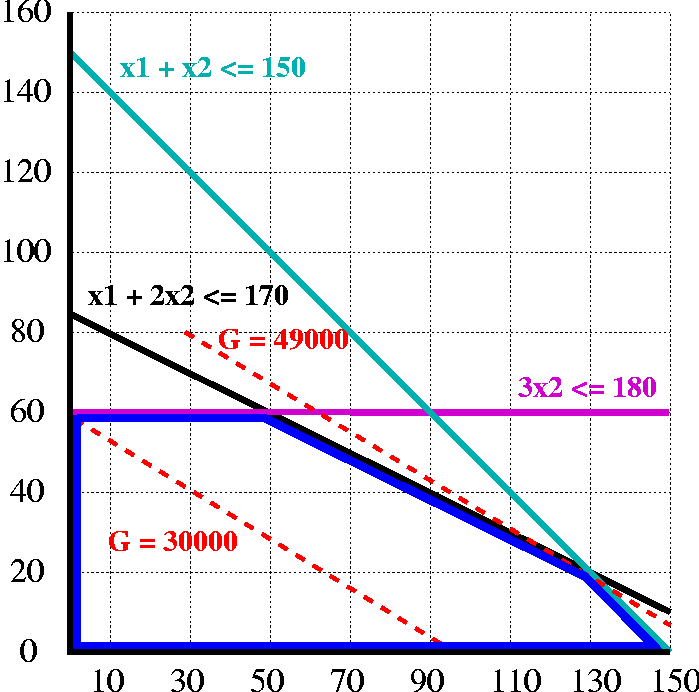
\includegraphics[scale=0.22]{Linear_programming_polytope.png}
\caption{problema de otimização resolvido com programação linear \cite{wiki:xxh}}
\label{fig:programacao linear}
\end{figure}
\bibliographystyle{plain}
\bibliography{pm.bib}
\end{document}
